\section{Secondary market analysis}
\label{sec:methods}
As part of our ongoing effort to understand how the mechanisms of Namecoin function, we want to understand how names move between users. In this section we attempt to quantify this movement of names. We explore multiple methods of detecting the sale of domains. Our basic scenario is that Alice owns the name `d/example' and Bob would like to purchase it from her. We explore various ways this sale can occur and how these sales can be detected.

\subsection{Atomic transfers}

\begin{figure*}
  \centering
  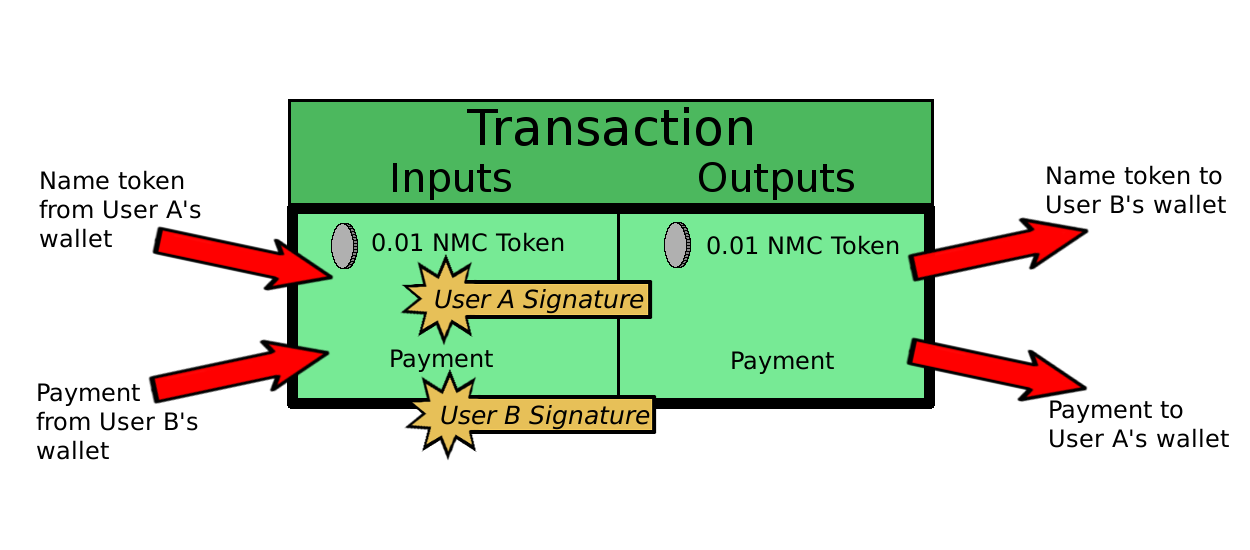
\includegraphics[width=0.9\textwidth]{figures/atomicTX}
  \caption{Functioning of atomic transactions}
  \label{fig:atomic}
\end{figure*}

The safest way to buy and sell Namecoin names is through the use of atomic transactions. We show how these transactions work in Figure \ref{fig:atomic}. In an atomic transaction, Alice and Bob make their exchange in a single transaction. In the simplest form of atomic name transfer, Bob creates a transaction which transfers his coins to Alice and transfers `d/example' to him. He then sends this transaction to Alice, the owner of the name, who verifies it, signs, and broadcasts the transaction to the blockchain. Both Alice and Bob's signatures are locked to the inputs and outputs of the transaction so it is impossible to spend . This transaction provides total safety to both Alice and Bob since either both the name and coins will be exchanged or nothing will. Although there is nothing inherently different looking about this transaction, there are a few possible techniques to detect them by implementation quirks.

The Namecoin client is a fairly underdeveloped piece of software and thus there is no built-in method of performing atomic transactions. In order to accomplish this task, the Namecoin RPC client must be used from the command line. In order to simplify this task, a Namecoin developer created ANTPY \cite{antyp}, a piece of software to automate the creation of atomic transactions. This software has the quirk that the buyer's payment goes to the address that the seller held the name in. To find these transactions we queried the blockchain for transactions with a NAME\_FIRSTUPDATE or NAME\_UPDATE input from the same address as a non name output. We then further reduced this set by eliminating transactions where the name stayed at the same address.

We searched throughout the history of the Namecoin block chain for transactions fitting this specification. Our query returned 13 transactions which we believe represent all transactions built by the ANTPY script. However this by no means represents all sales on the block chain. We next attempt to discover atomic transactions in a different way.

A implementation agnostic method for detecting atomic name transfers is to find transactions that clearly use change addresses. This occurs when there are two non-name outputs in a transaction that has a name input. In this case the buyer did not want to pay all of his input to the seller and thus kept some for himself. This leaves the transaction with 3 outputs. Under normal circumstances, name transactions will only have two outputs, a name output and a change address. Thus every transaction with three outputs is very likely an atomic name transfer.

We also search throughout the history of the Namecoin blockchain for transactions with obvious change addresses. We found 6 transactions fitting this form. However 5 of the 6 were detected by the previous specification.

The 18 atomic transactions which we detected are a lower bound for the number of name transfers. We are unable to query for all atomic transactions since if the buyer doesn't want any change from a purchase and the seller gives the buyer a new address to send payment to, the transaction is indistinguishable from a regular non-transferring name update.

\subsection{Deriving an upper bound on number of sales}

Following up on our lower bound from the previous section, we now derive an upper bound on the number of name sales using data from the blockchain. Whereas atomic transactions, could be recognized simply from the contents of a transaction, other name sale transactions are not recognizable. We would hope that we could detect changes in name ownership by looking at changes in which key owns a name. However, since the Namecoin client defaults to sending names to new addresses on update, there is no way to look at an update and tell whether or not a name is being transferred between owners.

In order to detect non-atomic transactions we must expand our view to the prior value of a name being updated. Certainly if the value does not change then the transaction is simply renewing the name, not transferring it. However considering all other transactions to be name transfers is far too conservative of a criterium. Users freely update the values of names whenever information in them becomes outdated and under the stated criterium this would all apply to be transfers. Thus it appears that there is not clear way to detect all name transfers.

\begin{figure}
  \centering
  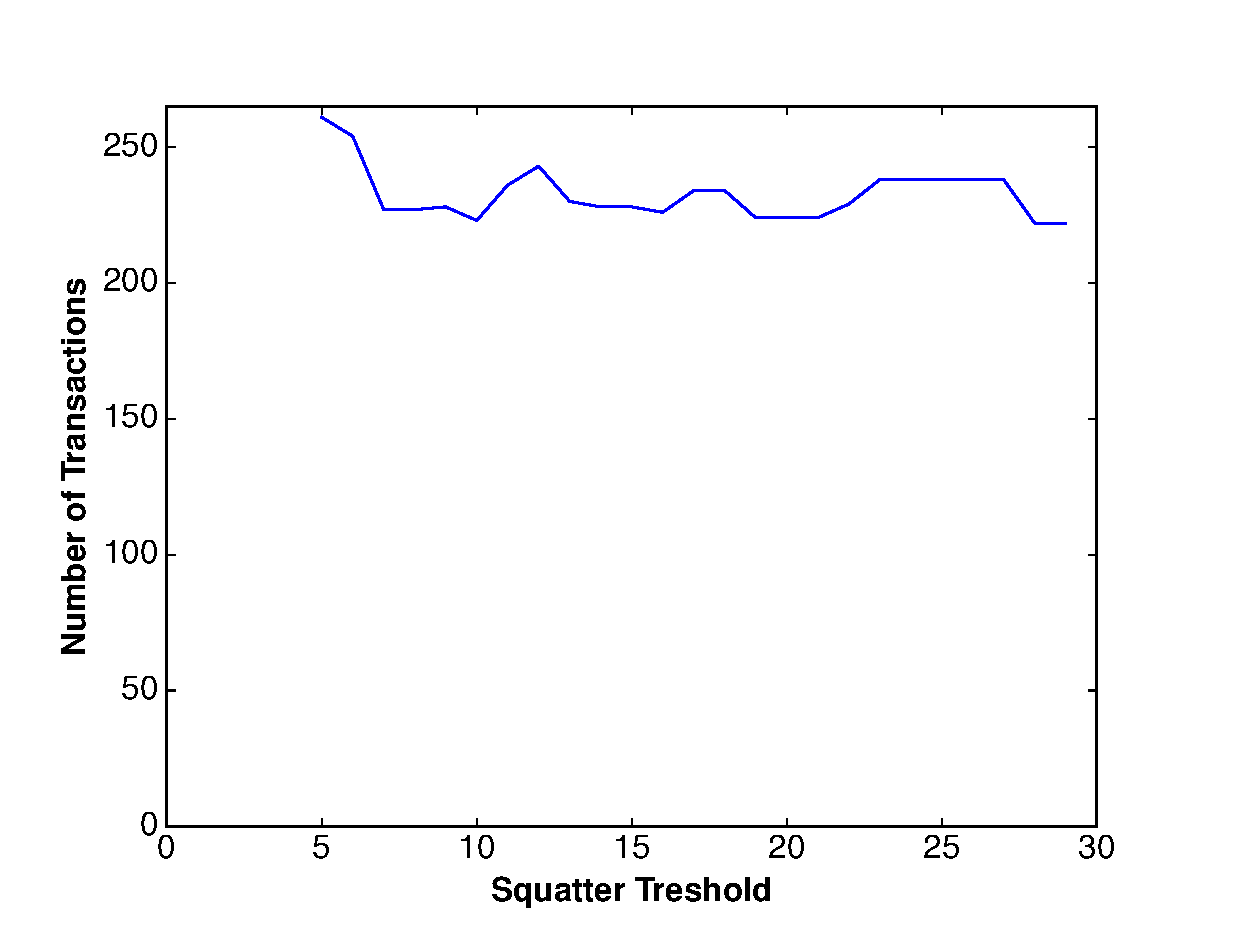
\includegraphics[width=0.9\columnwidth]{figures/transfers}
  \caption{Percent of names considered squatted}
  \label{fig:percentSquatter}
\end{figure}

Although we have eliminated the possibility of detecting non-atomic name transfers generally, there is an important subclass of these transactions which can still be detected, transfers from squatters to regular users. In the previous section we discussed our detection of squatters in the blockchain which produces a list of values which with a high probability belong to squatters. Detecting transfers from squatters by finding names that change from one of these values gives us an almost working strategy to detect transfers.

There are a few more ways we can eliminate possible transfers. Sometimes squatters update the value of their names, and thus a change from a squatter value may not represent the transfer of a name. To avoid picking up these updates as name transfers we restrict ourselves to selecting transactions that update the value of a name from a squatter value to a non-squatter value. Additionally if a name's value includes an info or email field and that stays the same in the updated value we can assume this is simply an update by the squatter. Although this criterium is certainly not perfect, we believe that it has a fairly high success rate in revealing overall trends in name transfers.

Applying this analysis at various squatter threshold values, we see that the total number of transactions detected holds at approximately 250 transactions. This value is likely an upper-bound since our criteria for reducing the number of transactions were quite conservative. 